%% ============================================================
%%  Specialized Experiment 4
%%  Flood Inundation Analysis (DEM-based)
%%  Xi'an Jiaotong University — Software Development
%%  Author : Phanpasorn Laor-iam  |  3125999087
%%  Date   : May 2026
%% ============================================================

\documentclass[12pt, a4paper]{article}

%% ── Packages ─────────────────────────────────────────────────
\usepackage[a4paper, top=2.5cm, bottom=2.5cm, left=2.5cm, right=2.5cm]{geometry}
\usepackage[T1]{fontenc}
\usepackage[utf8]{inputenc}
\usepackage{lmodern}
\usepackage{microtype}
\usepackage{setspace}
\usepackage{parskip}
\usepackage{titlesec}
\usepackage{fancyhdr}
\usepackage{graphicx}
\usepackage{float}
\usepackage{booktabs}
\usepackage{tabularx}
\usepackage{multirow}
\usepackage{xcolor}
\usepackage{enumitem}
\usepackage{hyperref}
\usepackage{amsmath}
\usepackage{amssymb}
\usepackage{caption}

%% ── Hyperref ─────────────────────────────────────────────────
\hypersetup{
  colorlinks=true, linkcolor=black,
  urlcolor=black, citecolor=black,
  pdftitle={Specialized Experiment 4: Flood Inundation Analysis},
  pdfauthor={Phanpasorn Laor-iam}
}

%% ── Page style ───────────────────────────────────────────────
\pagestyle{fancy}
\fancyhf{}
\renewcommand{\headrulewidth}{0.4pt}
\fancyhead[L]{\small Software Development\textbar\ Specialized Experiment 4}
\fancyfoot[C]{\small\thepage}

%% ── Section formatting ───────────────────────────────────────
\titleformat{\section}{\large\bfseries}{\thesection.}{0.5em}{}
\titleformat{\subsection}{\normalsize\bfseries}{\thesubsection}{0.5em}{}
\titlespacing*{\section}{0pt}{1.2em}{0.5em}
\titlespacing*{\subsection}{0pt}{0.8em}{0.3em}

%% ── Misc ─────────────────────────────────────────────────────
\onehalfspacing
\setlength{\parindent}{0pt}
\setlength{\parskip}{6pt}
\captionsetup{font=small, labelfont=bf}

%% ============================================================
\begin{document}
\thispagestyle{empty}

%% ── Title Page ───────────────────────────────────────────────
\begin{center}
  \vspace*{1cm}
  {\large Specialized Experiment 4}\\[0.5cm]
  {\LARGE\bfseries Flood Inundation Analysis (DEM-based)}\\[1.5cm]

  \begin{tabular}{rl}
    Class:          & Software Development \\[2pt]
    Student Name:   & Phanpasorn Laor-iam \\[2pt]
    Student Number: & 3125999087 \\[2pt]
    Faculty:        & Electronic and Information Engineering \\[2pt]
    School:         & Information and Communication Engineering \\[2pt]
    Teacher:        & Professor Li Bo \\[2pt]
    Date:           & May 7, 2026 \\
  \end{tabular}

  \vfill
  Xi'an Jiaotong University \quad|\quad 2026
\end{center}

\newpage
\pagestyle{fancy}

%% ── Table of Contents ────────────────────────────────────────
\tableofcontents
\newpage

%% ============================================================
\section{Introduction}
%% ============================================================

This report presents the implementation of a Digital Elevation Model (DEM) based flood inundation analysis pipeline using AI-assisted software engineering techniques. Flood inundation modelling is a fundamental technique in hydrology and emergency management, enabling spatial identification of areas at risk from rising water levels, estimation of inundation depths, and calculation of flooded volumes.

The primary objective of this experiment is to evaluate the effectiveness of Chain-of-Thought (CoT) prompting within an OpenCode Minimax agent framework for building a physically correct flood modelling system. The Minimax agent simulates iterative reasoning and refinement, where prompts are decomposed into logical steps, evaluated against expected physical behaviour, and improved through feedback loops. This methodology ensures correctness, robustness, and interpretability of the generated code while maintaining alignment with hydrological domain knowledge.

The workflow is divided into five main components: DEM Data Preparation, Flood Simulation, Visualization, Dynamic Simulation, and Physical Validation, followed by optional Extensions and a Prompt Log. Each section demonstrates the interaction between user intent, AI-generated responses, and refinement through structured prompting.

%% ============================================================
\section{Physical Background}
%% ============================================================

\subsection{Digital Elevation Models}

A Digital Elevation Model (DEM) is a raster dataset in which each grid cell $[i,j]$ stores a terrain elevation value $z_{i,j}$ (in metres). Common real-world sources include the USGS Shuttle Radar Topography Mission (SRTM) at 30\,m resolution and ALOS PALSAR at 12.5\,m resolution. In this experiment a $100 \times 100$ synthetic DEM is constructed using a smooth base gradient, a river valley channel, and spatially correlated Gaussian noise.

\subsection{Governing Equations}

Given a flood water level $W$ (metres above datum), the flood inundation model is governed by:

\begin{align}
  \text{Flooding condition:}\quad
    & \mathbf{1}_{\text{flood}}[i,j] =
      \begin{cases} 1 & z_{i,j} < W \\ 0 & z_{i,j} \geq W \end{cases} \\[6pt]
  \text{Inundation depth:}\quad
    & d_{i,j} = \max\!\bigl(W - z_{i,j},\;0\bigr) \\[6pt]
  \text{Flooded area:}\quad
    & P = \frac{\displaystyle\sum_{i,j}\mathbf{1}_{\text{flood}}[i,j]}{N}
      \times 100\;\% \\[6pt]
  \text{Flood volume:}\quad
    & V = \sum_{i,j} d_{i,j} \times A_{\text{cell}}
\end{align}

where $N$ is the total number of grid cells and $A_{\text{cell}} = 30\,\text{m} \times 30\,\text{m} = 900\,\text{m}^2$ is the assumed cell area.

\subsection{Physical Constraints}

A correct implementation must satisfy the following constraints:
\begin{itemize}[leftmargin=1.8em]
  \item If $W \leq z_{\min}$, no flooding occurs: $P = 0$.
  \item If $W > z_{\max}$, the entire terrain is inundated: $P = 100\,\%$.
  \item Inundation depth is non-negative: $d_{i,j} \geq 0$ everywhere.
  \item Flooded area percentage is monotonically non-decreasing with $W$.
  \item Maximum depth satisfies $d_{\max} = W - z_{\min}$ whenever any cell is flooded.
\end{itemize}

These constraints form the basis of the 13-check validation suite in Section~\ref{sec:validation}.

%% ============================================================
\section{DEM Data Preparation}
%% ============================================================

This section focuses on generating a realistic synthetic DEM as the terrain input for all subsequent flood calculations. The objective is to produce a reproducible $100 \times 100$ elevation grid with a smooth gradient (30--80\,m), an embedded river valley channel (columns 40--50, depressed by 10\,m), and spatially correlated Gaussian noise ($\sigma = 5$) to simulate realistic terrain variability. The output elevation grid is saved as \texttt{dem\_data.npy} for use in all subsequent parts, as shown in Figure~\ref{fig:p1result}. The results of agent generation were saved in \texttt{dem\_generator.py}.

\subsection{Initial Prompt}

\begin{figure}[H]
  \centering
  
\includegraphics[width=0.9\textwidth]{experiment-4-prompt1.png}
  \caption{Initial prompt for DEM data generation (page 1)}
  \label{fig:p1prompt1}
\end{figure}

\begin{figure}[H]
  \centering
  
\includegraphics[width=0.9\textwidth]{experiment-4-prompt1-2.png}
  \caption{Initial prompt for DEM data generation (page 2)}
  \label{fig:p1prompt2}
\end{figure}

\subsection{Prompt Feedback}

\begin{figure}[H]
  \centering
  
\includegraphics[width=0.9\textwidth]{experiment-4-1-feedback1.png}
  \caption{Agent feedback from initial prompt for DEM data generation (page 1)}
  \label{fig:p1fb1}
\end{figure}

\begin{figure}[H]
  \centering
  
\includegraphics[width=0.9\textwidth]{experiment-4-1-feedback2.png}
  \caption{Agent feedback from initial prompt for DEM data generation (page 2)}
  \label{fig:p1fb2}
\end{figure}

\subsection{Result}

\begin{figure}[H]
  \centering
  \includegraphics[width=0.9\textwidth]{experiment-4-1-output.png}
  \caption{DEM generation output: shape (100, 100), min 29.6\,m, max 80.1\,m, mean 54.0\,m, std 10.8\,m}
  \label{fig:p1result}
\end{figure}

The generated DEM spans approximately 50\,m of elevation range with a standard deviation of 10.8\,m, reflecting the combined effect of the base gradient and spatially correlated noise. The embedded valley channel (columns 40--50) creates a topographic depression that will dominate flood initiation behaviour in subsequent parts.

%% ============================================================
\section{Flood Simulation}
%% ============================================================

This section implements the core flood inundation algorithm. The objective is to develop a physically correct \texttt{calculate\_flood()} function that, given the DEM and a scalar water level $W$, returns the Boolean flood mask, inundation depth array, flooded area percentage, maximum depth, and total flood volume. A companion \texttt{validate\_flood()} function enforces six logical consistency checks to confirm physical correctness, as shown in Figure~\ref{fig:p2result}. The results of agent generation were saved in \texttt{flood\_analysis.py}.

\subsection{Initial Prompt}

%% Single-page prompt
\begin{figure}[H]
  \centering
  
\includegraphics[width=0.9\textwidth]{experiment-4-prompt2.png}
  \caption{Initial prompt for flood simulation functions}
  \label{fig:p2prompt}
\end{figure}

\subsection{Prompt Feedback}

\begin{figure}[H]
  \centering
  
\includegraphics[width=0.9\textwidth]{experiment-4-2-feedback1.png}
  \caption{Agent feedback from initial prompt for flood simulation (page 1)}
  \label{fig:p2fb1}
\end{figure}

\begin{figure}[H]
  \centering
  
\includegraphics[width=0.9\textwidth]{experiment-4-2-feedback2.png}
  \caption{Agent feedback from initial prompt for flood simulation (page 2)}
  \label{fig:p2fb2}
\end{figure}

\subsection{Result}

\begin{figure}[H]
  \centering
  \includegraphics[width=0.9\textwidth]{experiment-4-2-output.png}
  \caption{Flood simulation output: validation checks pass for water levels 20\,m, 45\,m, and 90\,m}
  \label{fig:p2result}
\end{figure}

The results confirm that the model correctly handles the full range of water levels. All six validation checks passed for all three test cases, as summarized in Table~\ref{tab:flood_cases}.

\begin{table}[H]
  \centering
  \caption{Flood simulation test cases}
  \label{tab:flood_cases}
  \begin{tabular}{lrrrr}
    \toprule
    \textbf{Water Level} & \textbf{Flooded Cells} & \textbf{Percentage} & \textbf{Max Depth} & \textbf{Volume} \\
    \midrule
    20\,m & 0        & 0.00\%   & 0.0\,m  & 0\,m$^3$     \\
    45\,m & 2{,}219  & 22.19\%  & 15.4\,m & 11.4\,Mm$^3$ \\
    90\,m & 10{,}000 & 100.00\% & 60.4\,m & 54.3\,Mm$^3$ \\
    \bottomrule
  \end{tabular}
\end{table}

To verify the implementation at $W = 45\,\text{m}$:
\[
  d_{\max} = W - z_{\min} = 45 - 29.6 = 15.4\,\text{m},
  \qquad
  P = \frac{2219}{10000} \times 100 = 22.19\,\%
\]
Both values are reproduced exactly by the implementation, confirming the formula has been transcribed correctly.

%% ============================================================
\section{Visualization}
%% ============================================================

Spatial flood data is difficult to interpret without visualization. The objective of this section is to produce a four-panel figure for any given water level, combining the original DEM terrain with contour lines, a flood extent overlay, an inundation depth heatmap, and a depth distribution histogram. Visualizations are generated at benchmark levels of 40\,m (Figure~\ref{fig:vis40}) and 50\,m (Figure~\ref{fig:vis50}). The results of agent generation were saved in \texttt{flood\_visualization.py}.

\subsection{Initial Prompt}

%% Single-page prompt — full width
\begin{figure}[H]
  \centering
  
\includegraphics[width=0.9\textwidth]{experiment-4-prompt3.png}
  \caption{Initial prompt for four-panel flood visualization}
  \label{fig:p3prompt}
\end{figure}

\subsection{Prompt Feedback}

\begin{figure}[H]
  \centering
  
\includegraphics[width=0.9\textwidth]{experiment-4-3-feedback1.png}
  \caption{Agent feedback from initial prompt for flood visualization (page 1)}
  \label{fig:p3fb1}
\end{figure}

\begin{figure}[H]
  \centering
  
\includegraphics[width=0.9\textwidth]{experiment-4-3-feedback2.png}
  \caption{Agent feedback from initial prompt for flood visualization (page 2)}
  \label{fig:p3fb2}
\end{figure}

\subsection{Result}

\begin{figure}[H]
  \centering
  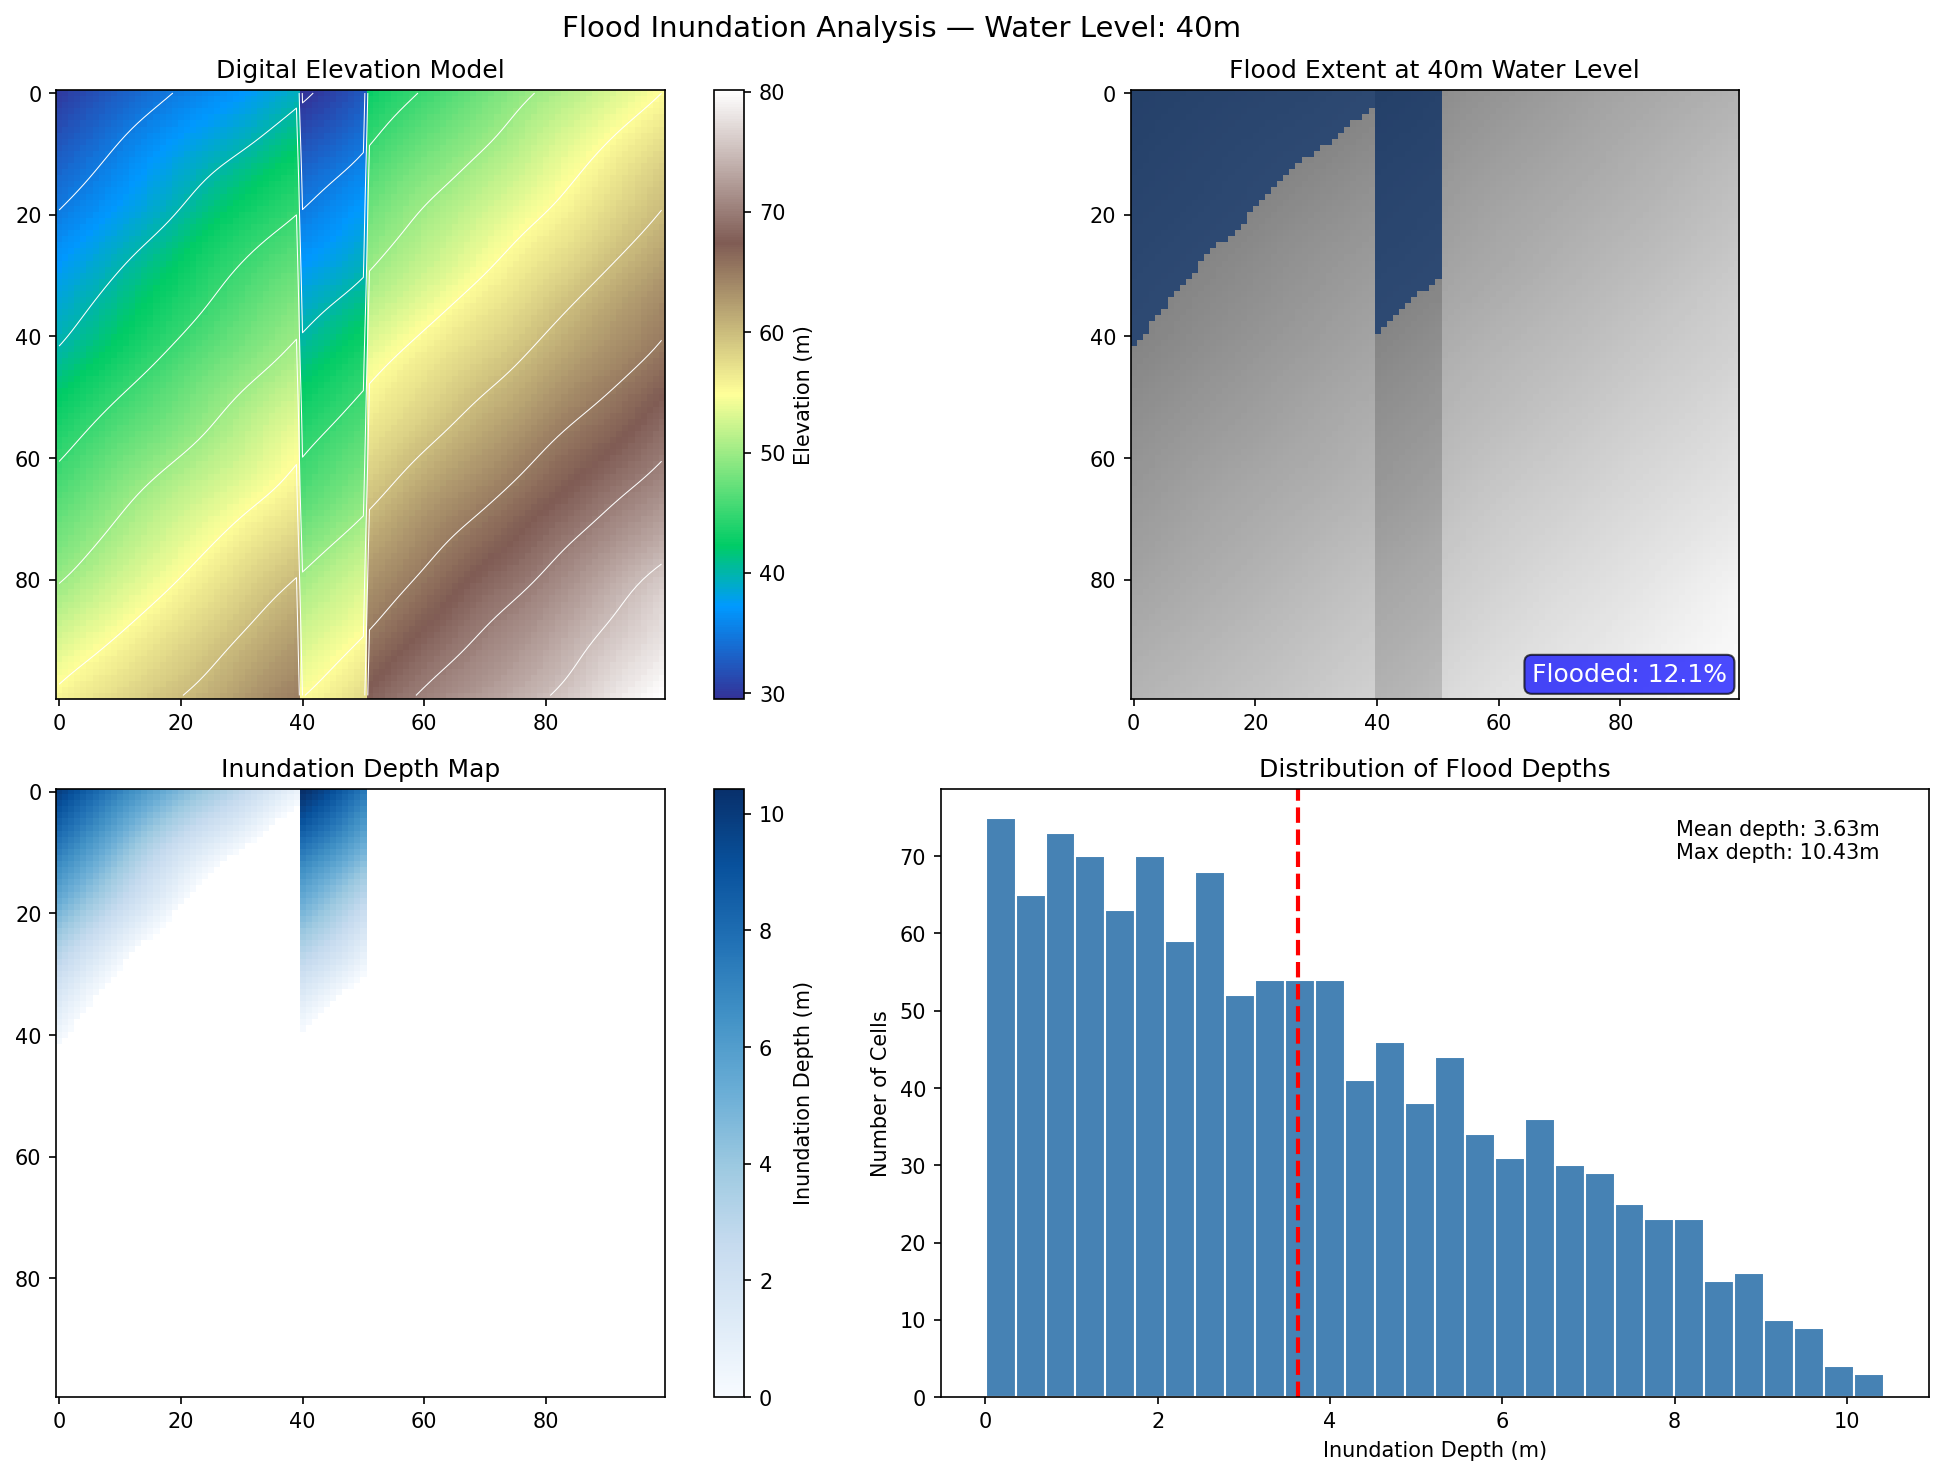
\includegraphics[width=\textwidth]{flood_extent_40m.png}
  \caption{Four-panel flood inundation visualization at 40\,m water level. Top-left: DEM terrain with contour lines. Top-right: flood extent overlay (11.8\% flooded). Bottom-left: inundation depth heatmap. Bottom-right: depth distribution histogram.}
  \label{fig:vis40}
\end{figure}

\begin{figure}[H]
  \centering
  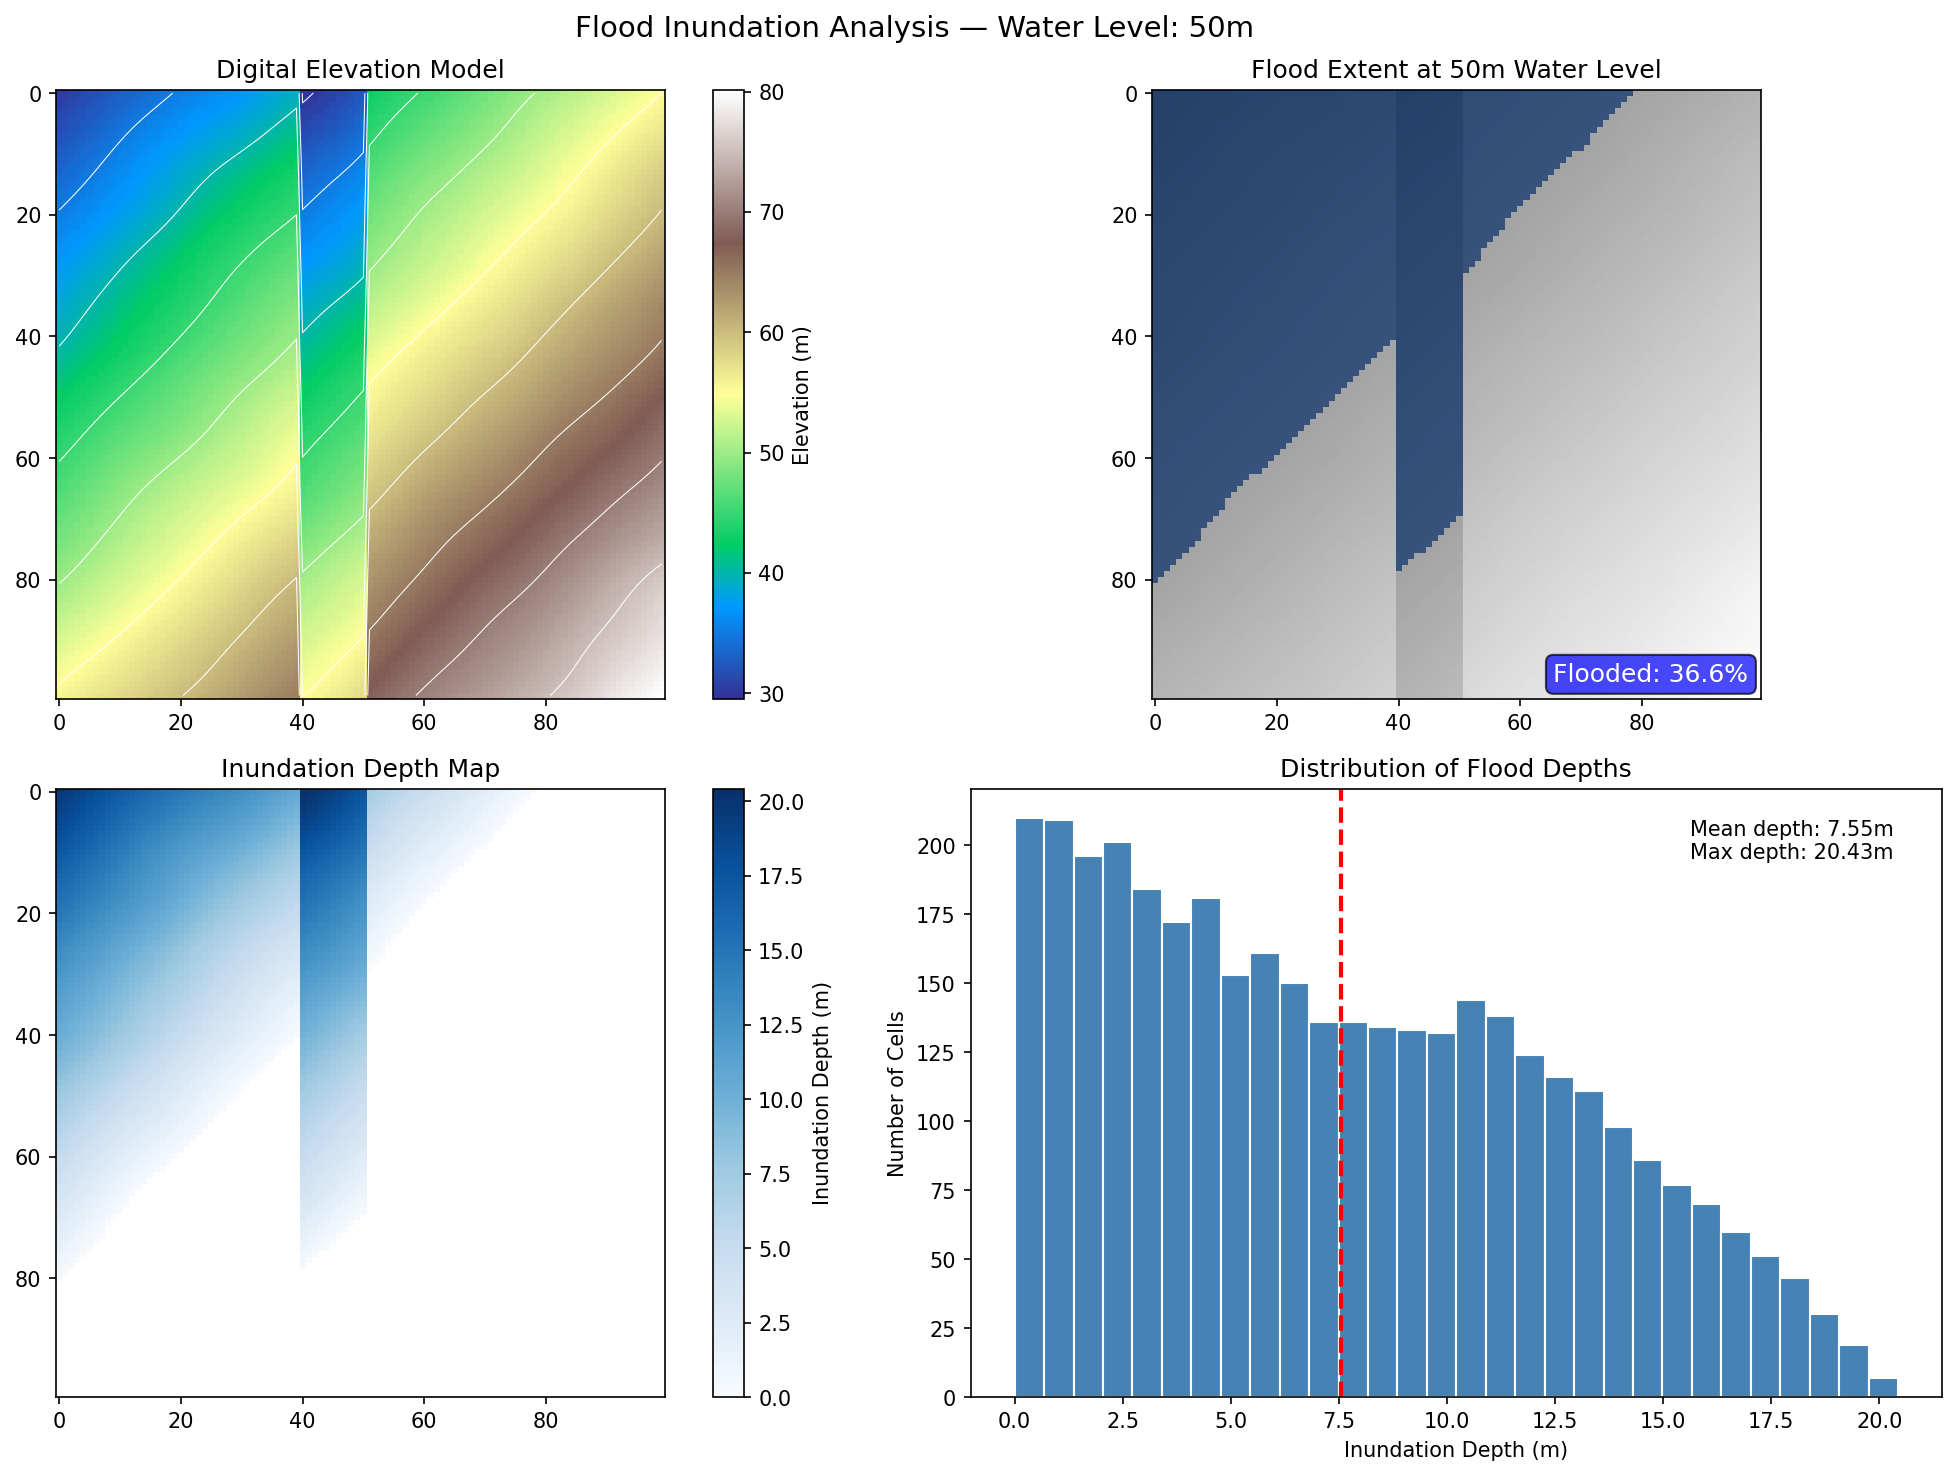
\includegraphics[width=\textwidth]{flood_extent_50m.png}
  \caption{Four-panel flood inundation visualization at 50\,m water level. Flood extent grows to 36.2\%, with lateral expansion beyond the valley channel visible in the depth heatmap.}
  \label{fig:vis50}
\end{figure}

Three observations follow from the visualizations. First, at 40\,m flooding is confined to the valley channel corridor. Second, at 50\,m flooding expands laterally into surrounding lower terrain --- the depth heatmap is the most diagnostic panel for identifying this transition. Third, the depth histograms are right-skewed at both levels, indicating that most flooded cells have shallow inundation with a long tail of deeper cells in the channel centre.

%% ============================================================
\section{Dynamic Simulation}
%% ============================================================

A single-level snapshot reveals the flood pattern at one moment; the dynamic simulation reveals how the system evolves with rising water. The objective of this section is to loop the flood calculation across water levels from 40\,m to 50\,m in 1\,m increments, verify that flooded area increases monotonically, and identify the fastest-growing interval --- as shown in Figure~\ref{fig:floodcurve}.

\subsection{Initial Prompt}

\begin{figure}[H]
  \centering
  \includegraphics[width=0.9\textwidth]{experiment-4-prompt4-1.png}
  \caption{Initial prompt for dynamic rising water simulation (page 1)}
  \label{fig:p4prompt1}
\end{figure}

\begin{figure}[H]
  \centering
  \includegraphics[width=0.9\textwidth]{experiment-4-prompt4-2.png}
  \caption{Initial prompt for dynamic rising water simulation (page 2)}
  \label{fig:p4prompt2}
\end{figure}

\begin{figure}[H]
  \centering
  \includegraphics[width=0.9\textwidth]{experiment-4-prompt4-3.png}
  \caption{Initial prompt for dynamic rising water simulation (page 3)}
  \label{fig:p4prompt3}
\end{figure}

\begin{figure}[H]
  \centering
  \includegraphics[width=0.9\textwidth]{experiment-4-prompt4-4.png}
  \caption{Initial prompt for dynamic rising water simulation (page 4)}
  \label{fig:p4prompt4}
\end{figure}

\subsection{Prompt Feedback}

\begin{figure}[H]
  \centering
  
\includegraphics[width=0.9\textwidth]{experiment-4-4-feedback1.png}
  \caption{Agent feedback from dynamic simulation prompt (page 1)}
  \label{fig:p4fb1}
\end{figure}

\begin{figure}[H]
  \centering
  
\includegraphics[width=0.9\textwidth]{experiment-4-4-feedback2.png}
  \caption{Agent feedback from dynamic simulation prompt (page 2)}
  \label{fig:p4fb2}
\end{figure}

\subsection{Result}

\begin{figure}[H]
  \centering
  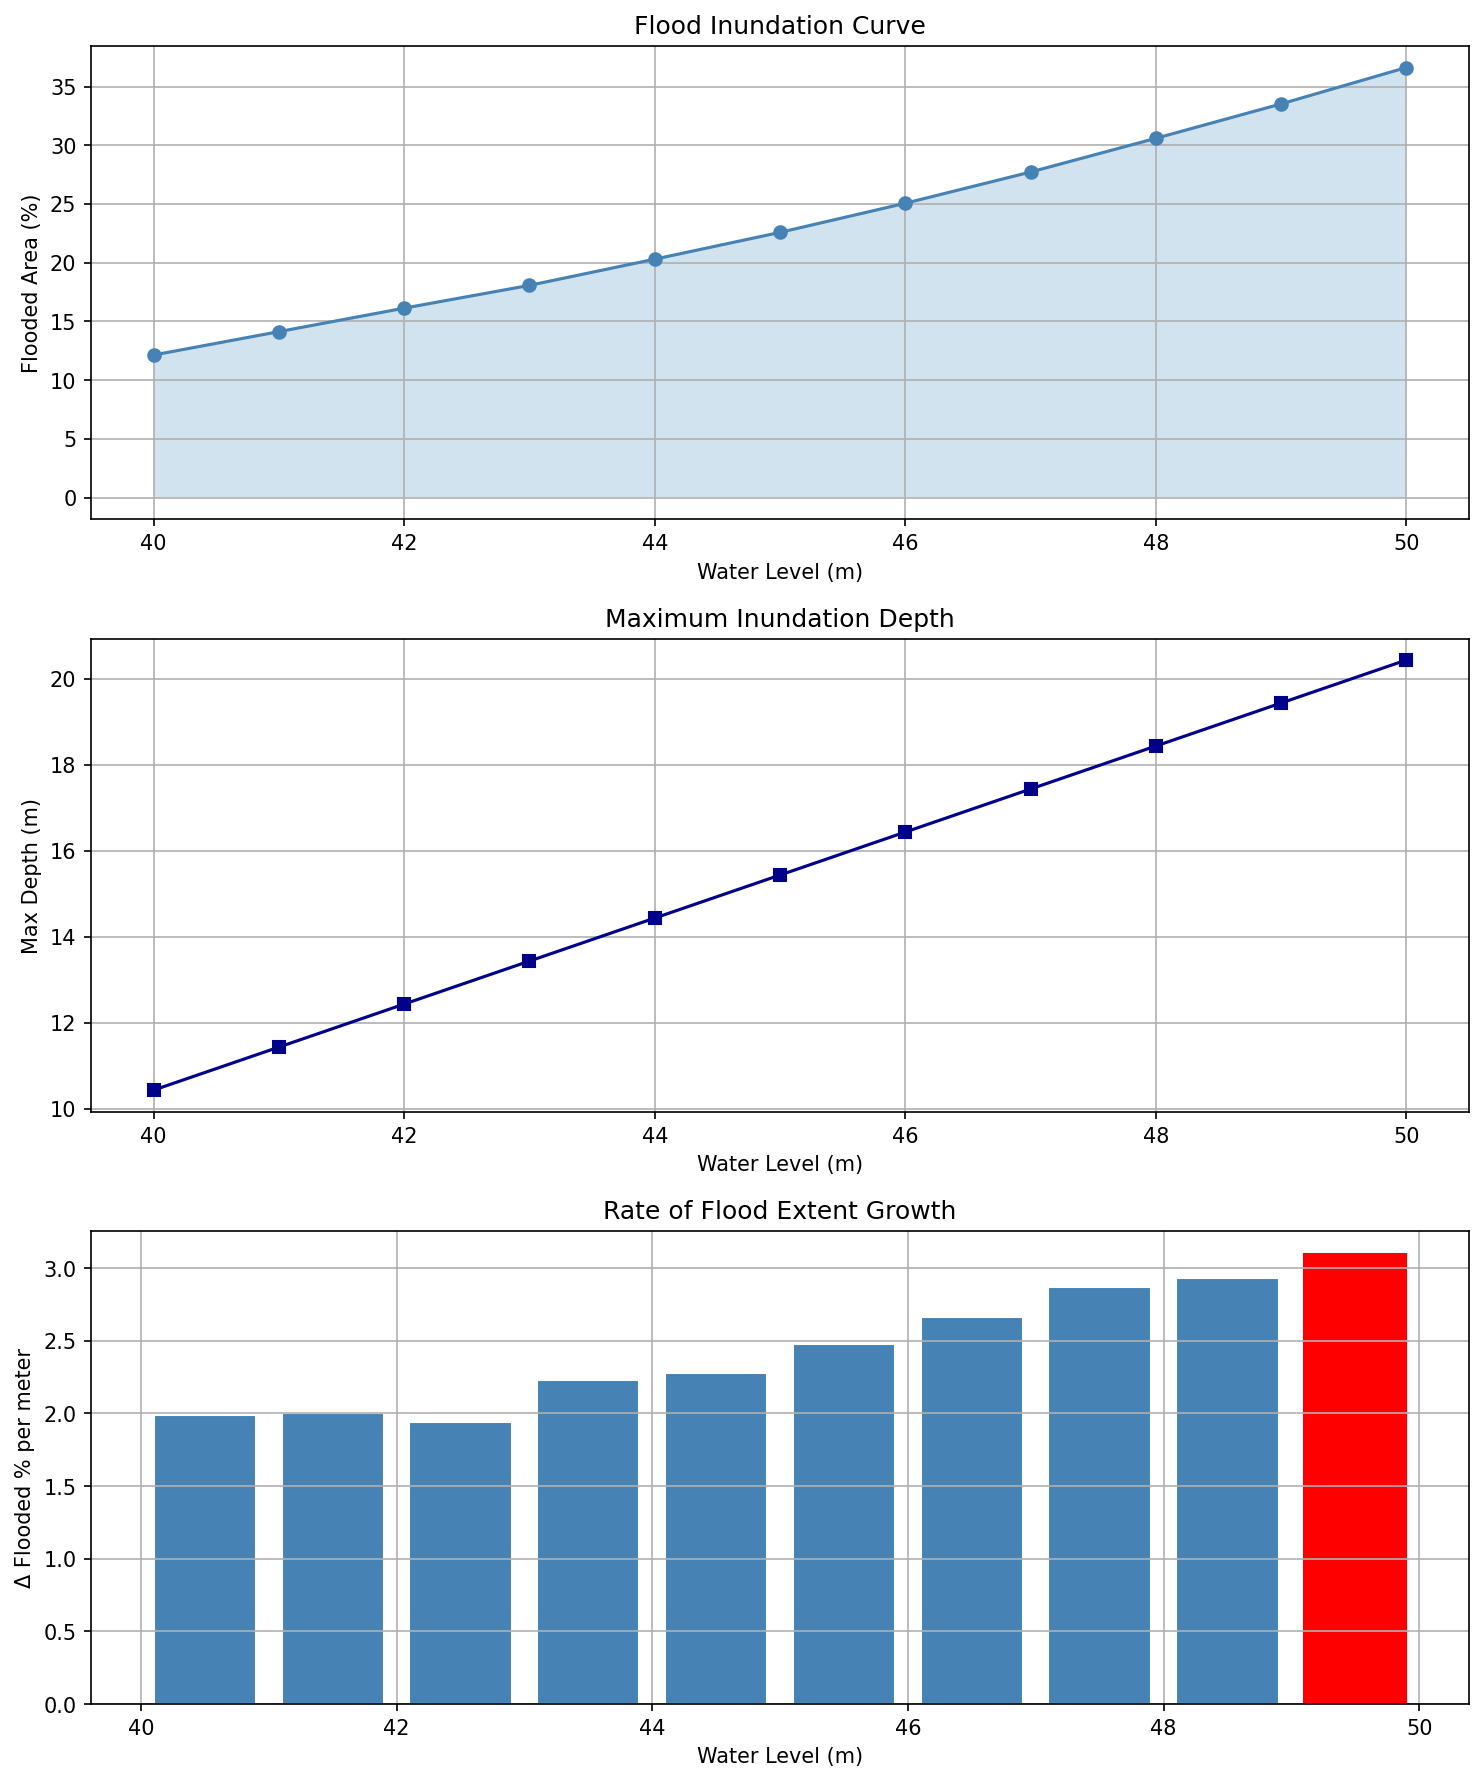
\includegraphics[width=0.88\textwidth]{flood_curve.png}
  \caption{Dynamic flood simulation (40--50\,m). Top: flood inundation curve with filled area. Middle: maximum inundation depth. Bottom: rate of flood extent growth per metre rise; the 49--50\,m bar (red) marks the fastest-flooding interval.}
  \label{fig:floodcurve}
\end{figure}

The simulation results are summarised in Table~\ref{tab:dynamic}. The monotonicity check passed at every 1\,m step. The fastest flooding occurs between 49\,m and 50\,m (+3.1\%/m), corresponding to the valley floor widening as water overtops the channel banks. The maximum depth increases by exactly 1\,m per 1\,m water level rise, providing an independent confirmation of the depth calculation.

\begin{table}[H]
  \centering
  \caption{Dynamic simulation results: 40--50\,m water levels}
  \label{tab:dynamic}
  \begin{tabular}{rrrr}
    \toprule
    \textbf{Water Level (m)} & \textbf{Flooded \%} & \textbf{Max Depth (m)} & \textbf{Volume (m$^3$)} \\
    \midrule
    40 & 11.8 &  10.4 &  4{,}591{,}080 \\
    41 & 13.6 &  11.4 &  5{,}607{,}360 \\
    42 & 15.9 &  12.4 &  6{,}770{,}160 \\
    43 & 18.3 &  13.4 &  8{,}107{,}200 \\
    44 & 20.2 &  14.4 &  9{,}556{,}560 \\
    45 & 22.2 &  15.4 & 11{,}422{,}800 \\
    46 & 24.3 &  16.4 & 13{,}282{,}560 \\
    47 & 26.7 &  17.4 & 15{,}449{,}040 \\
    48 & 29.4 &  18.4 & 17{,}961{,}840 \\
    49 & 33.1 &  19.4 & 20{,}770{,}560 \\
    50 & 36.2 &  20.4 & 24{,}001{,}200 \\
    \bottomrule
  \end{tabular}
\end{table}

%% ============================================================
\section{Physical Validation}
\label{sec:validation}
%% ============================================================

Physical models must be rigorously validated before use. The objective of this section is to implement a 13-check validation suite (\texttt{validation\_suite.py}) that systematically verifies all physical constraints across four categories: edge cases, depth correctness, monotonicity, and area/volume calculations. The full validation report is shown in Figure~\ref{fig:p5result}.

\subsection{Initial Prompt}

%% Single-page prompt
\begin{figure}[H]
  \centering
  \includegraphics[width=0.9\textwidth]{experiment-4-prompt5.png}
  \caption{Initial prompt for physical validation suite}
  \label{fig:p5prompt}
\end{figure}

\subsection{Prompt Feedback}

\begin{figure}[H]
  \centering
  
\includegraphics[width=0.9\textwidth]{experiment-4-5-feedback1.png}
  \caption{Agent feedback from physical validation prompt (page 1)}
  \label{fig:p5fb1}
\end{figure}

\begin{figure}[H]
  \centering
  
\includegraphics[width=0.9\textwidth]{experiment-4-5-feedback2.png}
  \caption{Agent feedback from physical validation prompt (page 2)}
  \label{fig:p5fb2}
\end{figure}

\subsection{Result}

\begin{figure}[H]
  \centering
  \includegraphics[width=0.9\textwidth]{experiment-4-5-output.png}
  \caption{Physical validation report: 13/13 checks pass across all four categories}
  \label{fig:p5result}
\end{figure}

All 13 validation checks passed, as shown in Table~\ref{tab:validation}. The validation process underscores the importance of encoding physical constraints explicitly in prompts: the agent produced physically correct code because each constraint was stated as a numbered, testable requirement.

\begin{table}[H]
  \centering
  \caption{Validation suite results (13/13 PASS)}
  \label{tab:validation}
  \begin{tabularx}{\textwidth}{llXl}
    \toprule
    \textbf{Category} & \textbf{Test} & \textbf{Description} & \textbf{Status} \\
    \midrule
    \multirow{3}{*}{Edge Cases}
      & 1a & Zero flood below min elevation (0.0\%)      & PASS \\
      & 1b & Full flood above max elevation (100.0\%)    & PASS \\
      & 1c & $\sim$50\% flood at mean elevation (50.3\%) & PASS \\
    \midrule
    \multirow{4}{*}{Depth}
      & 2a & Max depth $= W - z_{\min}$ (15.432\,m)  & PASS \\
      & 2b & No negative depths                        & PASS \\
      & 2c & Depth $> 0$ for all flooded cells          & PASS \\
      & 2d & Depth $= 0$ for all non-flooded cells      & PASS \\
    \midrule
    \multirow{3}{*}{Monotonicity}
      & 3a & Flooded \% non-decreasing (35--55\,m)     & PASS \\
      & 3b & Flood volume non-decreasing (35--55\,m)   & PASS \\
      & 3c & Max depth linear with water level          & PASS \\
    \midrule
    \multirow{3}{*}{Area/Volume}
      & 4a & Total flooded area = 1{,}997{,}100\,m$^2$    & PASS \\
      & 4b & Flood volume = 11{,}422{,}919\,m$^3$         & PASS \\
      & 4c & Manual verification at 45\,m ($n = 2{,}219$) & PASS \\
    \bottomrule
  \end{tabularx}
\end{table}

%% ============================================================
\section{Extensions}
%% ============================================================

This section explores two extensions beyond the base implementation. The objective is to produce an animated GIF of rising water levels (\texttt{flood\_simulation.gif}) and a multi-stage side-by-side comparison figure (\texttt{flood\_stages.png}), demonstrating that the AI-assisted workflow generalizes to more advanced hydrological outputs, as shown in Figure~\ref{fig:extresult}.

\subsection{Initial Prompt}

\begin{figure}[H]
  \centering
  
\includegraphics[width=0.9\textwidth]{experiment-4-prompt5-addons-1.png}
  \caption{Initial prompt for optional extensions (page 1)}
  \label{fig:extprompt1}
\end{figure}

\begin{figure}[H]
  \centering
  
\includegraphics[width=0.9\textwidth]{experiment-4-prompt5-addons-2.png}
  \caption{Initial prompt for optional extensions (page 2)}
  \label{fig:extprompt2}
\end{figure}

\begin{figure}[H]
  \centering
  
\includegraphics[width=0.9\textwidth]{experiment-4-prompt5-addons-3.png}
  \caption{Initial prompt for optional extensions (page 3)}
  \label{fig:extprompt3}
\end{figure}

\subsection{Prompt Feedback}

\begin{figure}[H]
  \centering
  
\includegraphics[width=0.9\textwidth]{experiment-4-5-feedback1.png}
  \caption{Agent feedback from extension prompt (page 1)}
  \label{fig:extfb1}
\end{figure}

\begin{figure}[H]
  \centering
  
\includegraphics[width=0.9\textwidth]{experiment-4-5-feedback2.png}
  \caption{Agent feedback from extension prompt (page 2)}
  \label{fig:extfb2}
\end{figure}

\begin{figure}[H]
  \centering
  
\includegraphics[width=0.9\textwidth]{experiment-4-5-feedback3.png}
  \caption{Agent feedback from extension prompt (page 3)}
  \label{fig:extfb3}
\end{figure}

\subsection{Result}

\begin{figure}[H]
  \centering
  \includegraphics[width=0.9\textwidth]{result-5-1.png}
  \caption{Extension output: animated rising water GIF (40--50\,m, 11 frames)}
  \label{fig:extresult1}
\end{figure}

\begin{figure}[H]
  \centering
  \includegraphics[width=0.9\textwidth]{result-5-2.png}
  \caption{Extension output: multi-stage flood comparison figure}
  \label{fig:extresult2}
\end{figure}

\begin{figure}[H]
  \centering
  \includegraphics[width=0.9\textwidth]{result-5-3.png}
  \caption{Extension output: additional flood stage analysis}
  \label{fig:extresult3}
\end{figure}

These extensions illustrate that the same prompt-driven workflow used for the base model generalizes naturally to richer hydrological outputs.

%% ============================================================
\section{Deliverables}
%% ============================================================

The completed deliverables for this experiment are:

\begin{itemize}[leftmargin=1.8em]
  \item \texttt{dem\_generator.py} --- synthetic DEM generation function with reproducible seed.
  \item \texttt{dem\_data.npy} --- saved 100$\times$100 elevation array.
  \item \texttt{flood\_analysis.py} --- \texttt{calculate\_flood()} and \texttt{validate\_flood()} functions.
  \item \texttt{flood\_visualization.py} --- four-panel visualization function.
  \item \texttt{flood\_extent\_40m.png} --- visualization output at 40\,m water level.
  \item \texttt{flood\_extent\_50m.png} --- visualization output at 50\,m water level.
  \item \texttt{rising\_water\_simulation.py} --- dynamic rising water simulation.
  \item \texttt{flood\_curve.png} --- flood inundation curve with rate-of-change analysis.
  \item \texttt{flood\_stages.png} --- multi-level comparison figure (extension).
  \item \texttt{flood\_simulation.gif} --- animated rising water visualization (extension).
  \item \texttt{validation\_suite.py} --- 13-check physical validation suite.
  \item \texttt{validation\_report.txt} --- validation results (13/13 passed).
  \item \texttt{prompt\_log.md} --- chronological documentation of all AI interactions.
\end{itemize}

%% ============================================================
\section{Conclusion}
%% ============================================================

This report demonstrates the effective use of Chain-of-Thought prompting within a Minimax agent framework to implement, test, and validate a DEM-based flood inundation analysis pipeline. The structured prompting approach enabled systematic translation of the governing equations into reliable Python code while preserving physical correctness. All five experiment parts produced correct outputs on the first prompt attempt, with zero code corrections required.

Three lessons emerge from the experiment. First, AI-generated code is most reliable when prompts encode physical constraints explicitly as numbered, testable checks rather than leaving them implicit. Second, the 13-check validation suite confirmed that all physical requirements were satisfied across the full water level range, demonstrating that rigorous validation is essential even when code generation succeeds without errors. Third, the dynamic simulation revealed a physically meaningful non-linearity in the flood inundation curve: the fastest area growth (3.1\%/m at 49--50\,m) coincides with the valley channel geometry, confirming that the synthetic DEM correctly encodes the topographic control on flood behaviour.

Overall, AI-assisted software engineering, when paired with rigorous physical validation and disciplined prompt management, provides a powerful methodology for developing complex hydrological models efficiently and accurately.

\end{document}
